\section{Sequence Diagrams}

The previous section outlined the functions of the system. Each of these 
functions are now to be ``converted'' into set of objects and interactions that 
might be implemented. A sequence diagram is ``one way of describing a journey 
through a system'' \citep{lunn03}.

\subsection{Single Week Cluster and Analysis (Weekly Basis)}
Figure \ref{fig:singleweekly} highlights the sequence of events that make up 
the clustering of data and analysing the clusters upon a weekly basis. This 
sequence diagram assumes that only one KML file will be given. 

Once clustered, the analysis only would be required to highlight the usage 
differences for the clusters that had been previously formed. An example of 
usage differences could be the number of events that occurred in one cluster 
versus another cluster, such as the number of 3G drops. 

Obviously as this is only a single week analysis then comparisons to other 
week's clusters can not be made.

Once the analysis has been completed, the results are written to a Javascript 
Object Notation (JSON) file and a new output KML file. This process was 
described in figure \ref{fig:UCAnalyseData}.

% Landscape page
\begin{landscape}
  % Center image
  \centering 
  \begin{figure}
    \centering
      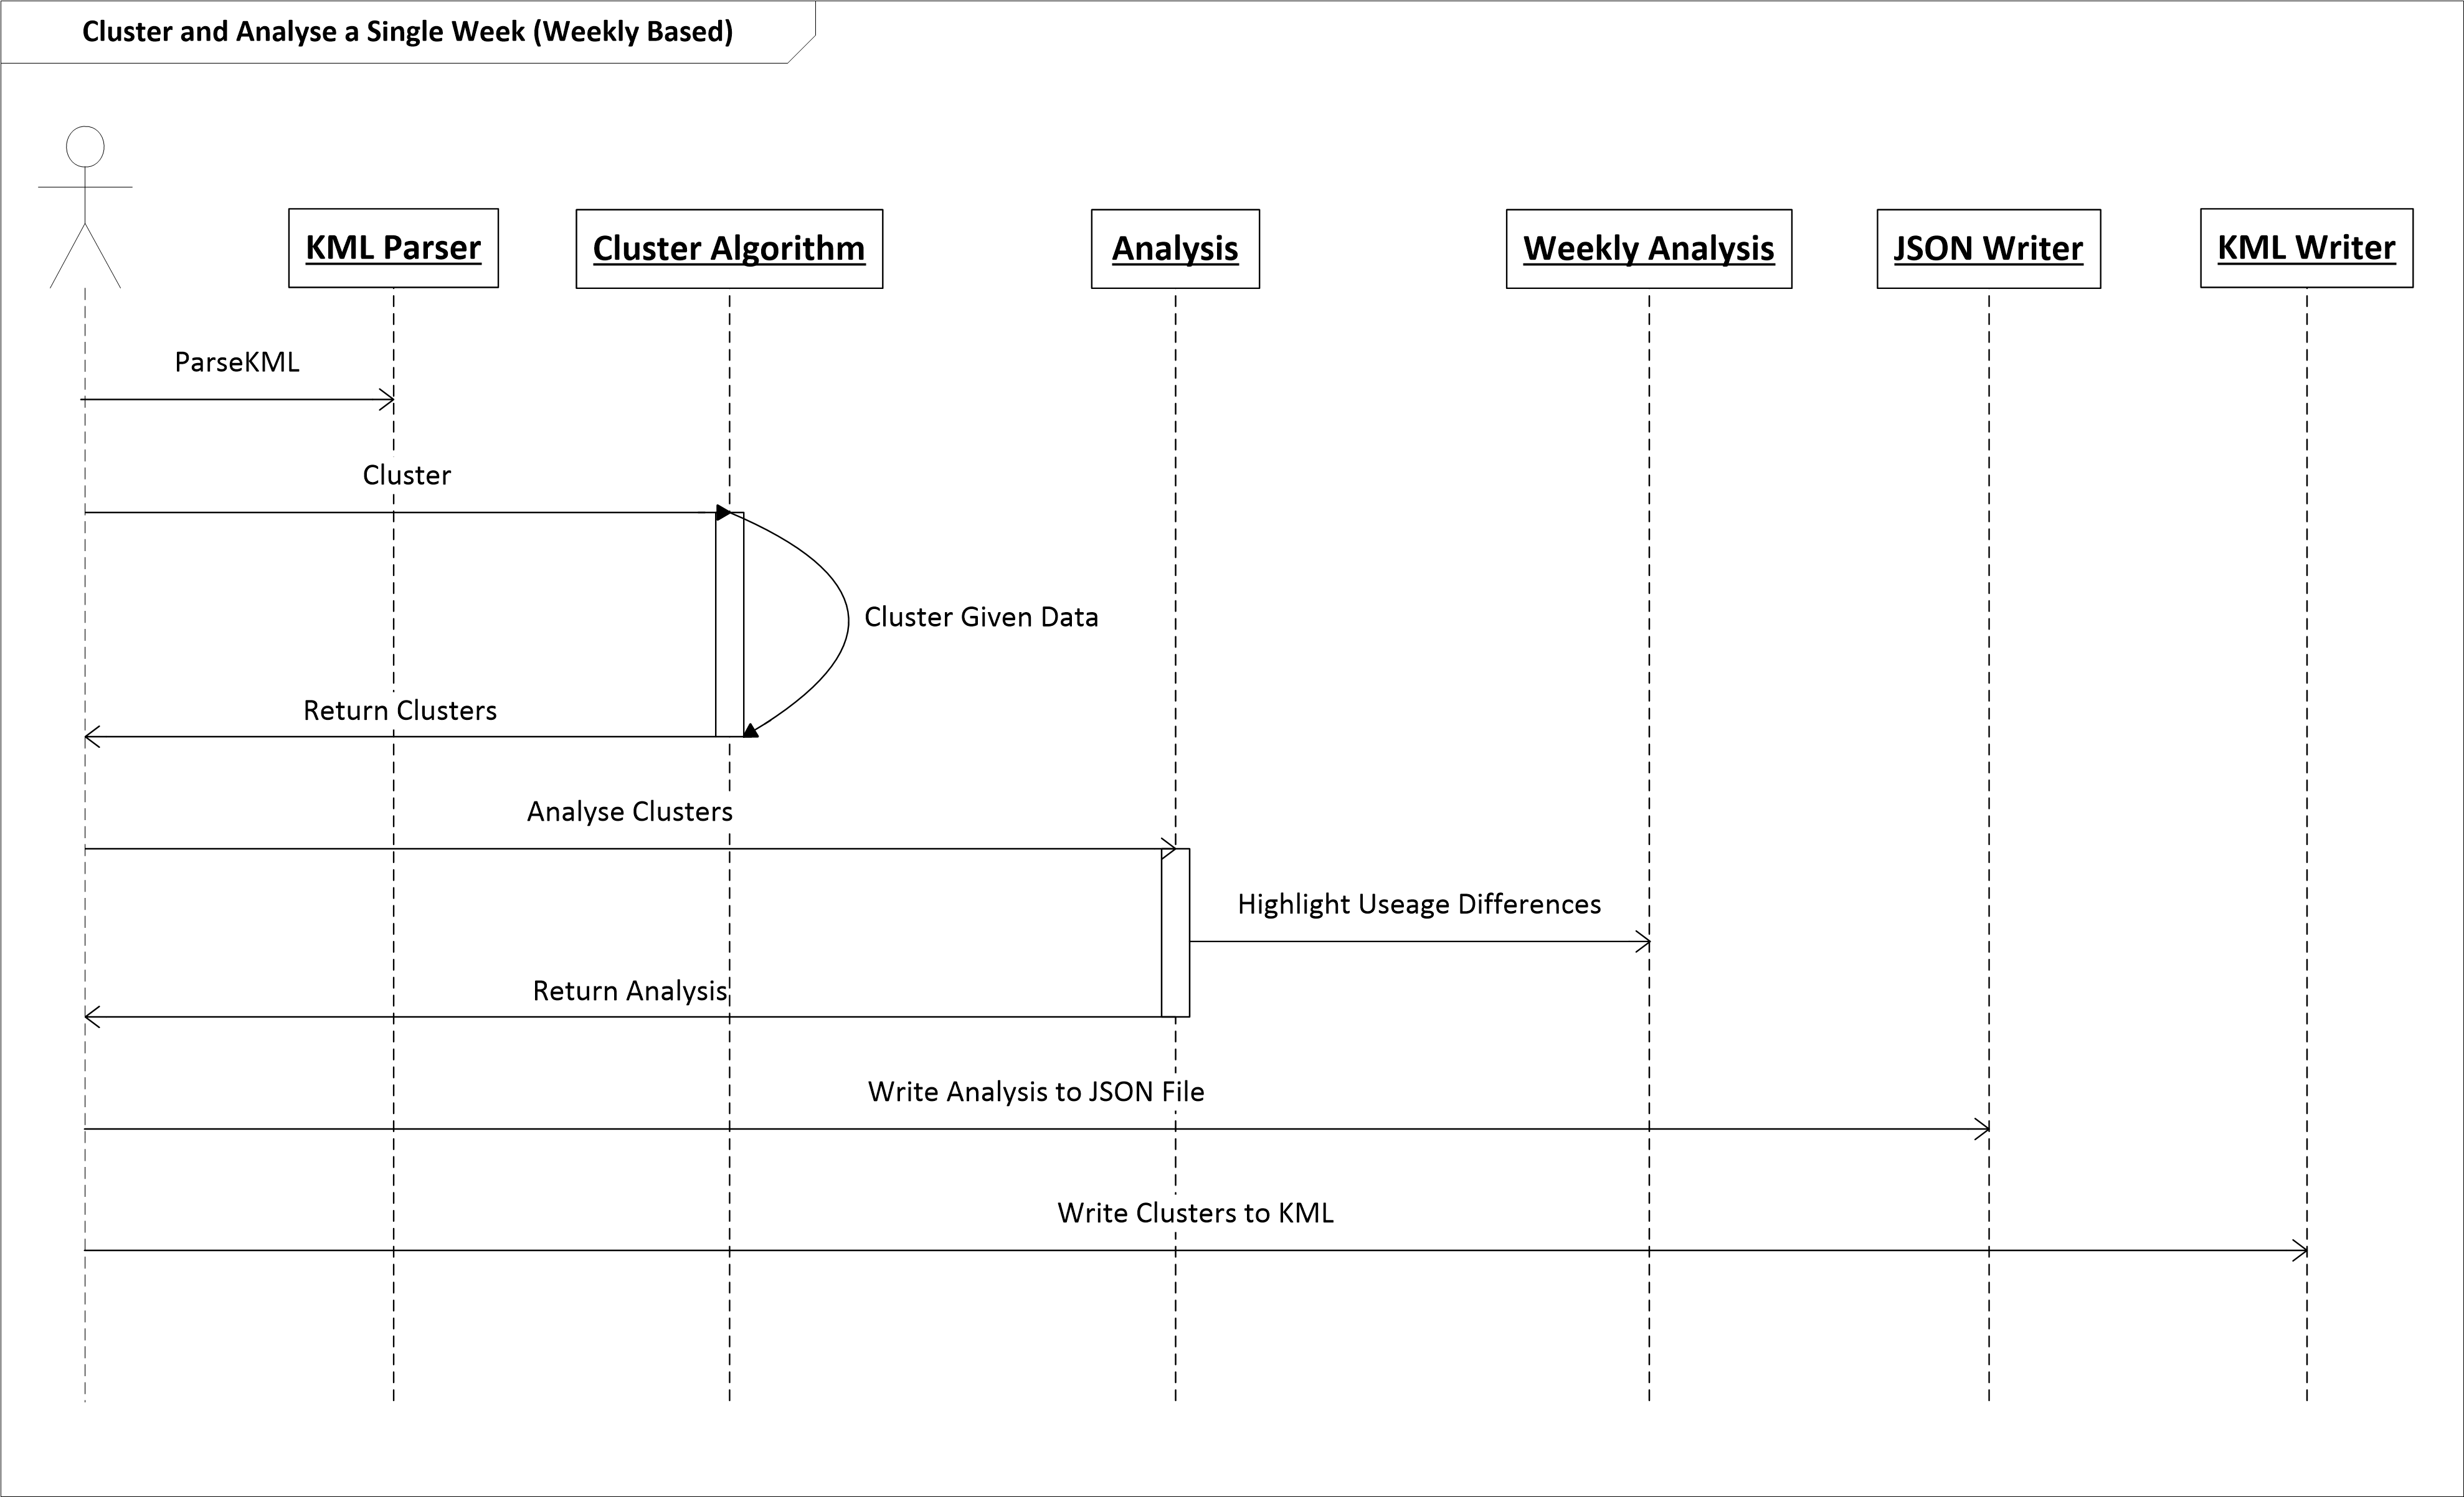
\includegraphics[scale=0.8]{chapter7/sequence_diagrams/single_week_cluster_weekly.png}
      \caption[Sequence diagram of a single week being clustered]
              {Sequence diagram of a single week being clustered and analysed 
              upon a weekly basis.}
      \label{fig:singleweekly}
  \end{figure}
\end{landscape}


\newpage
\subsection{Single Week Cluster and Analysis (Product Basis)}
Figure \ref{fig:singleproduct} highlights the sequence of events that make up 
the clustering of data and analysing the clusters upon a product basis.

As with the previous diagram, the tool would only be required to highlight the 
usage differences for the clusters that had been previously formed. However upon 
closer inspection, the Analysis event interacts with a `Product Analysis' event 
rather than the `Weekly Analysis' event that was found within the last diagram.

This highlights the only difference in the sequence of events for the weekly 
based analysis and the product based analysis.

As previously mentioned, once the analysis has been completed, the results are 
written to a JSON file and a new output KML file (see figure 
\ref{fig:UCAnalyseData} for more details).

% Landscape page
\begin{landscape}
  % Center image
  \centering 
  \begin{figure}
    \centering
      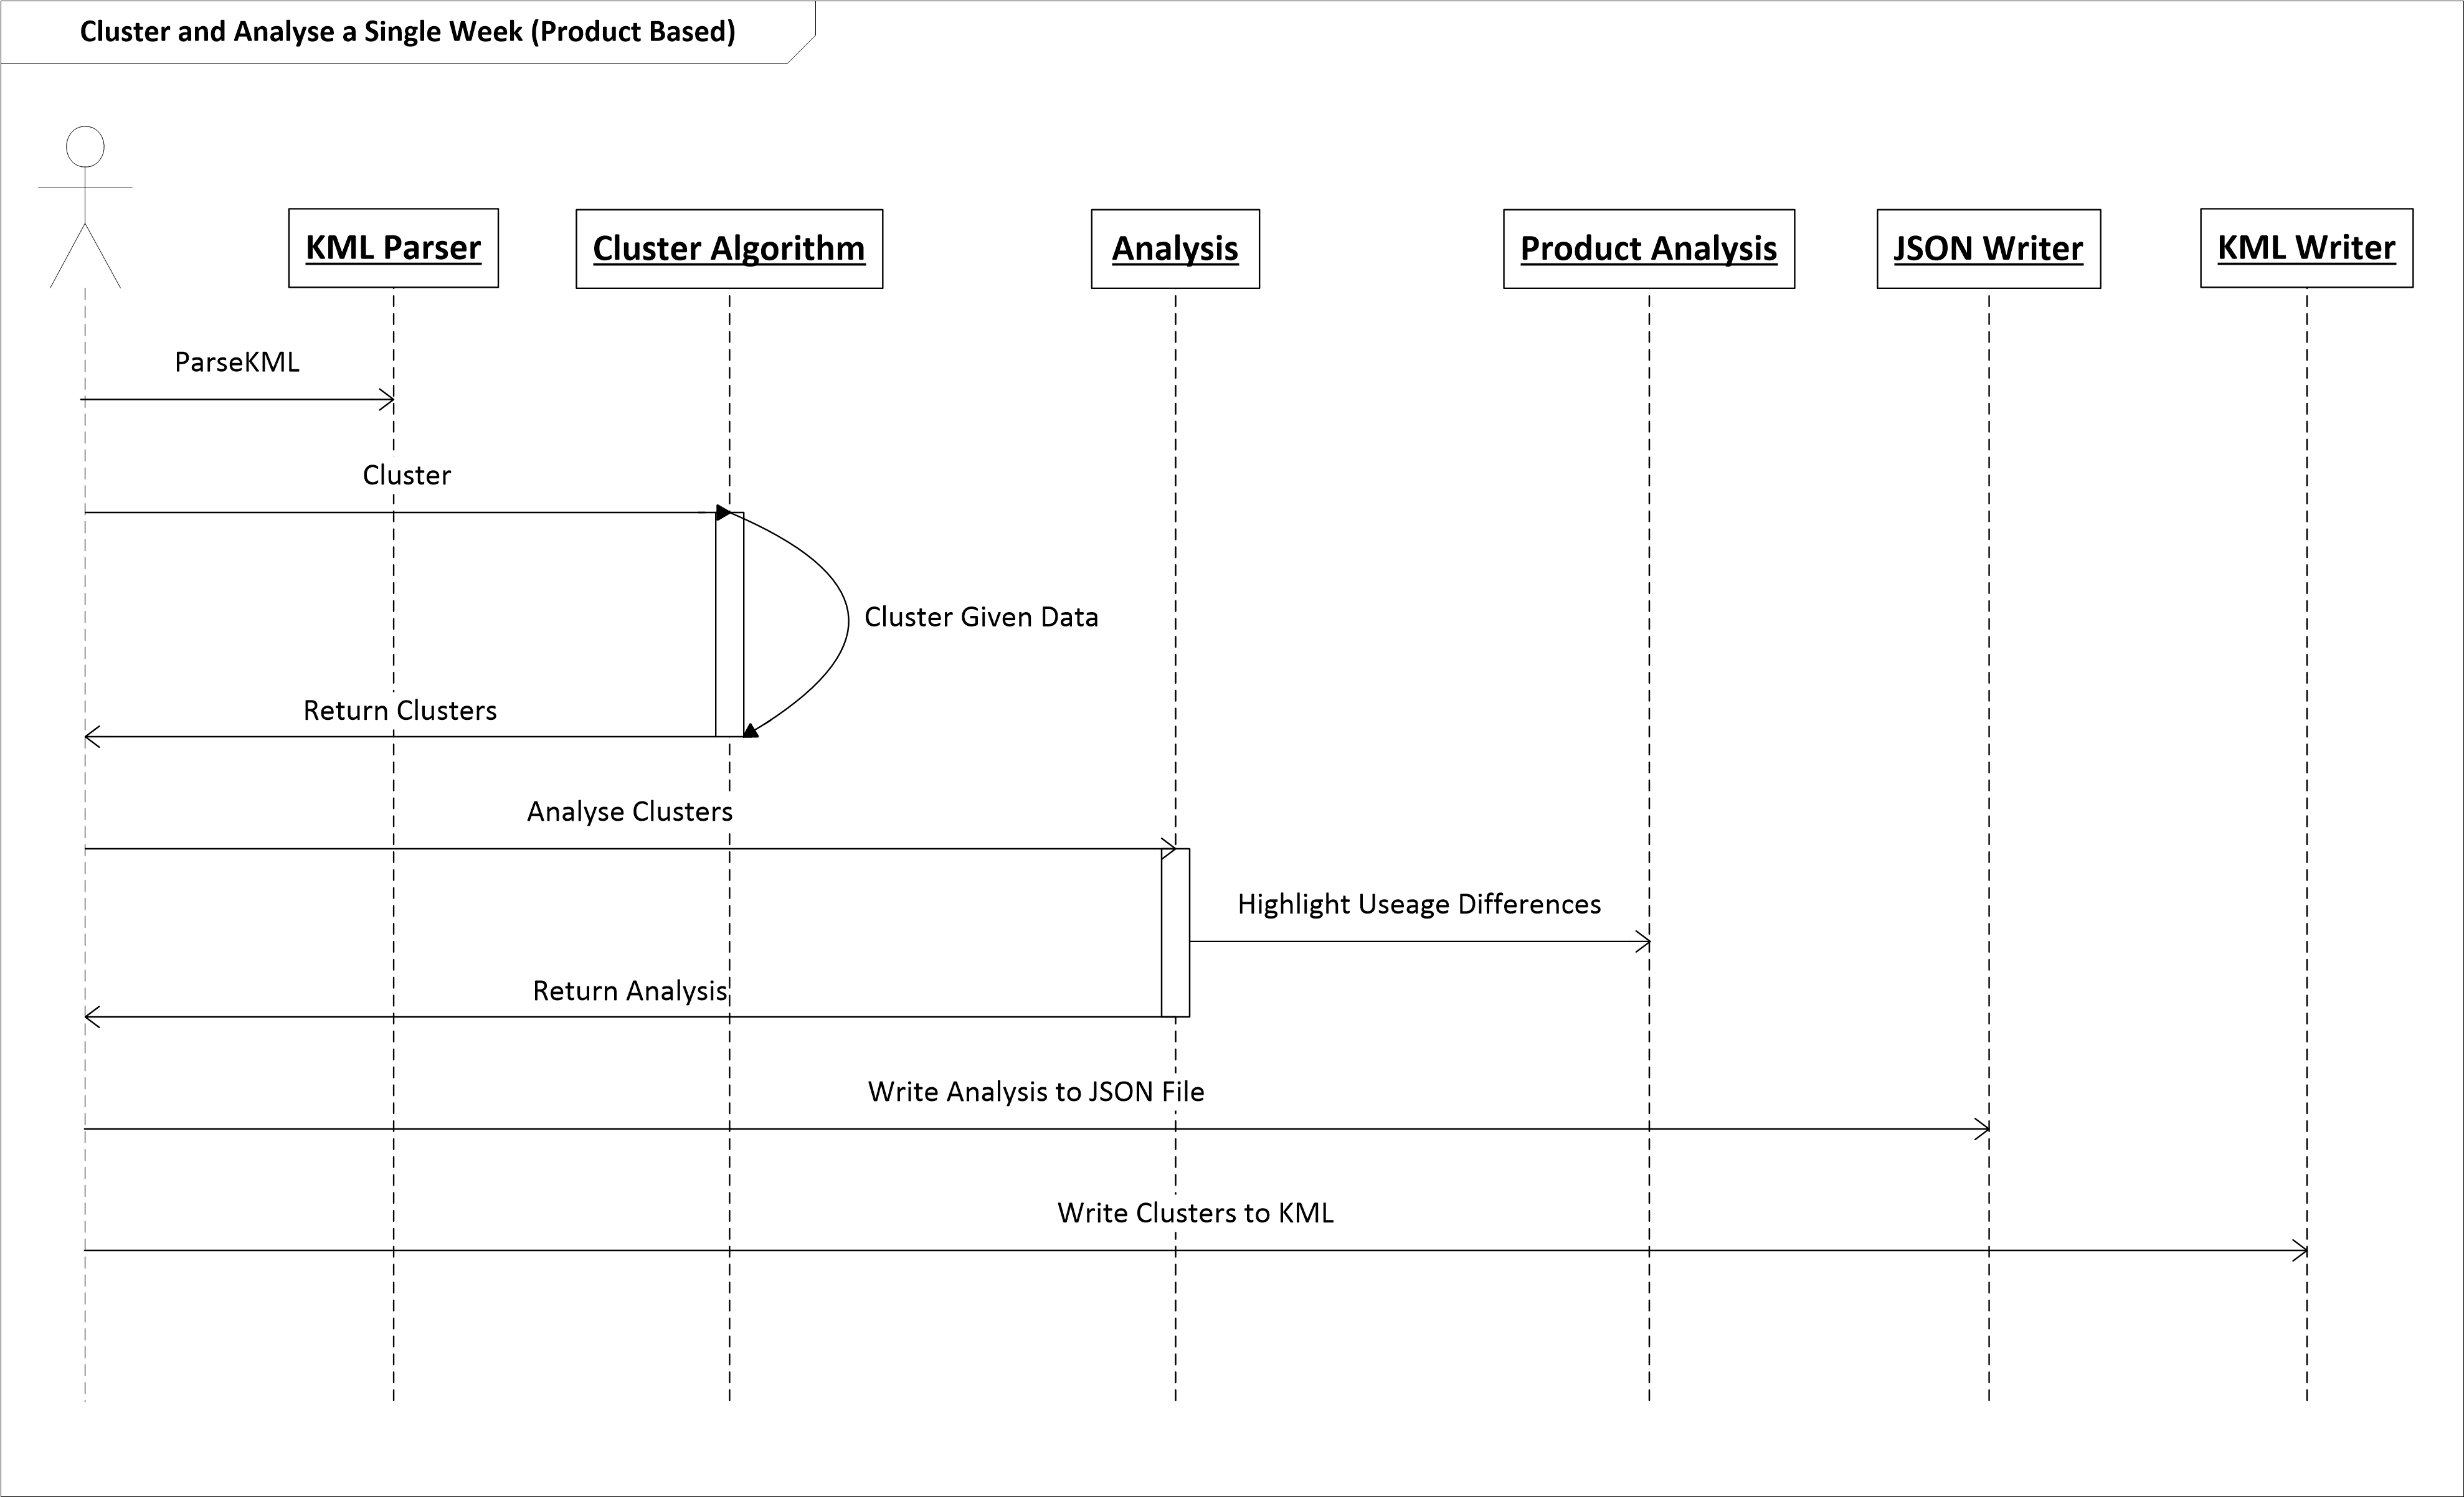
\includegraphics[scale=0.8]{chapter7/sequence_diagrams/single_week_cluster_product.png}
      \caption[Sequence diagram of a single week being clustered]
              {Sequence diagram of a single week being clustered and analysed 
              upon a product basis.}
      \label{fig:singleproduct}
  \end{figure}
\end{landscape}


\newpage
\subsection{Multi-Week Cluster and Analysis (Weekly Basis)}
Figure \ref{fig:multiweekly} highlights the sequence of events that make up 
the clustering of data and analysing the clusters upon a weekly basis.

The diagram is largely the same as the single file process, however the changes 
occur within the analysis stage of the process. The analysis event has to 
perform a number of additional analysis objectives before being able to save 
the data.

Firstly the process must highlight the differences in cluster coverings. For 
example week X may have events in clusters one to five, where as week Y may 
only have events in clusters one to three. 

Secondly, as well as presence, the process must also highlight changes to each 
cluster in real terms, such as the number increases and decreases upon a weekly 
basis. This is referred to as cluster density within the diagram.

Finally, the process must as highlight specific usage differences, such as an 
increase in 2G drops within cluster two. However this is the same as seen in 
the previous diagrams.


\afterpage{
  % Flush earlier floats (otherwise order might not be correct)
  \clearpage
  % Landscape page
  \begin{landscape}
    % Center image
    \centering 
    \begin{figure}
      \centering
        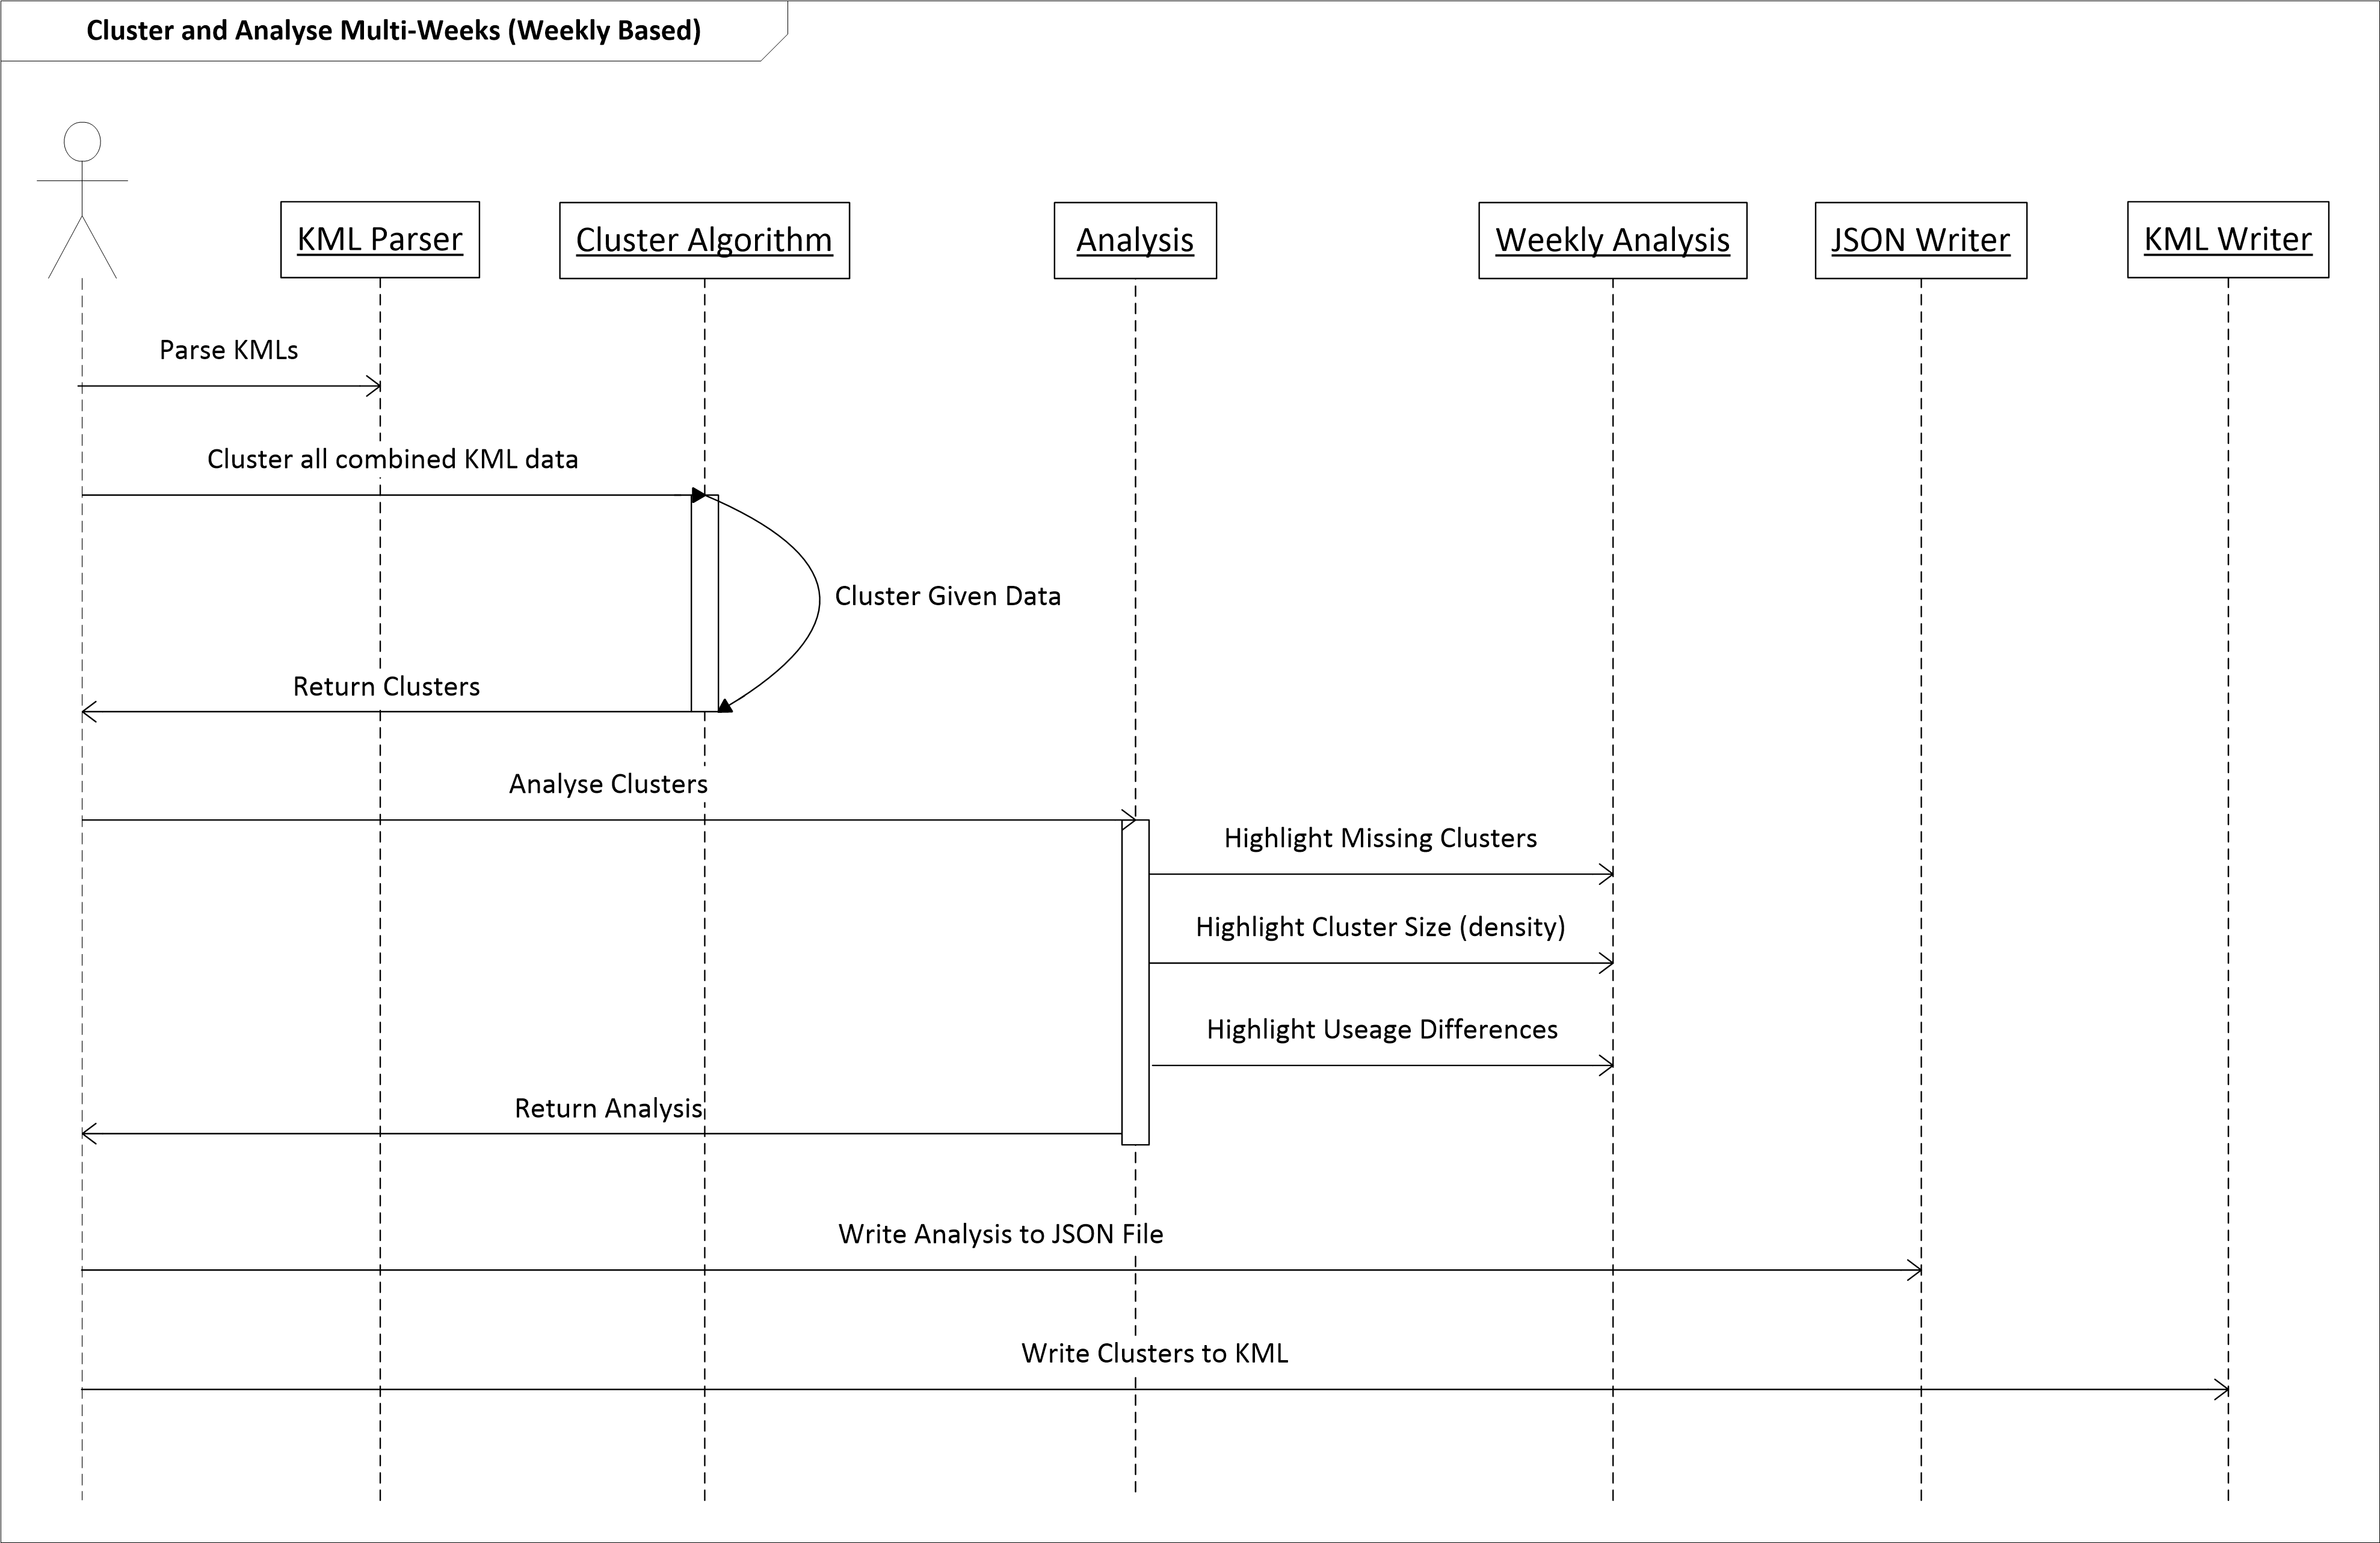
\includegraphics[scale=0.75]{chapter7/sequence_diagrams/multi_week_cluster_weekly.png}
        \caption[Sequence diagram of a multi-week being clustered]
                {Sequence diagram of a multi-week being clustered and analysed 
                upon a weekly basis.}
        \label{fig:multiweekly}
    \end{figure}
  \end{landscape}
  % Flush page
  \clearpage
}


\newpage
\subsection{Multi-Week Cluster and Analysis (Product Basis)}
Figure \ref{fig:multiproduct} highlights the sequence of events that make up 
the clustering of data and analysing the clusters upon a product basis.

The diagram is largely the same as the previous multi-week process, however the 
only change is that the pivot point is upon a product basis rather than a 
weekly-basis. For example device X may have events in clusters one to five, 
where as device Y may only have events in clusters one to three. 

As previously mentioned in all the diagrams, once the analysis has been 
completed, the results are written to a JSON file and a new output KML file.

\afterpage{
  % Flush earlier floats (otherwise order might not be correct)
  \clearpage
  % Landscape page
  \begin{landscape}
    % Center image
    \centering 
    \begin{figure}
      \centering
        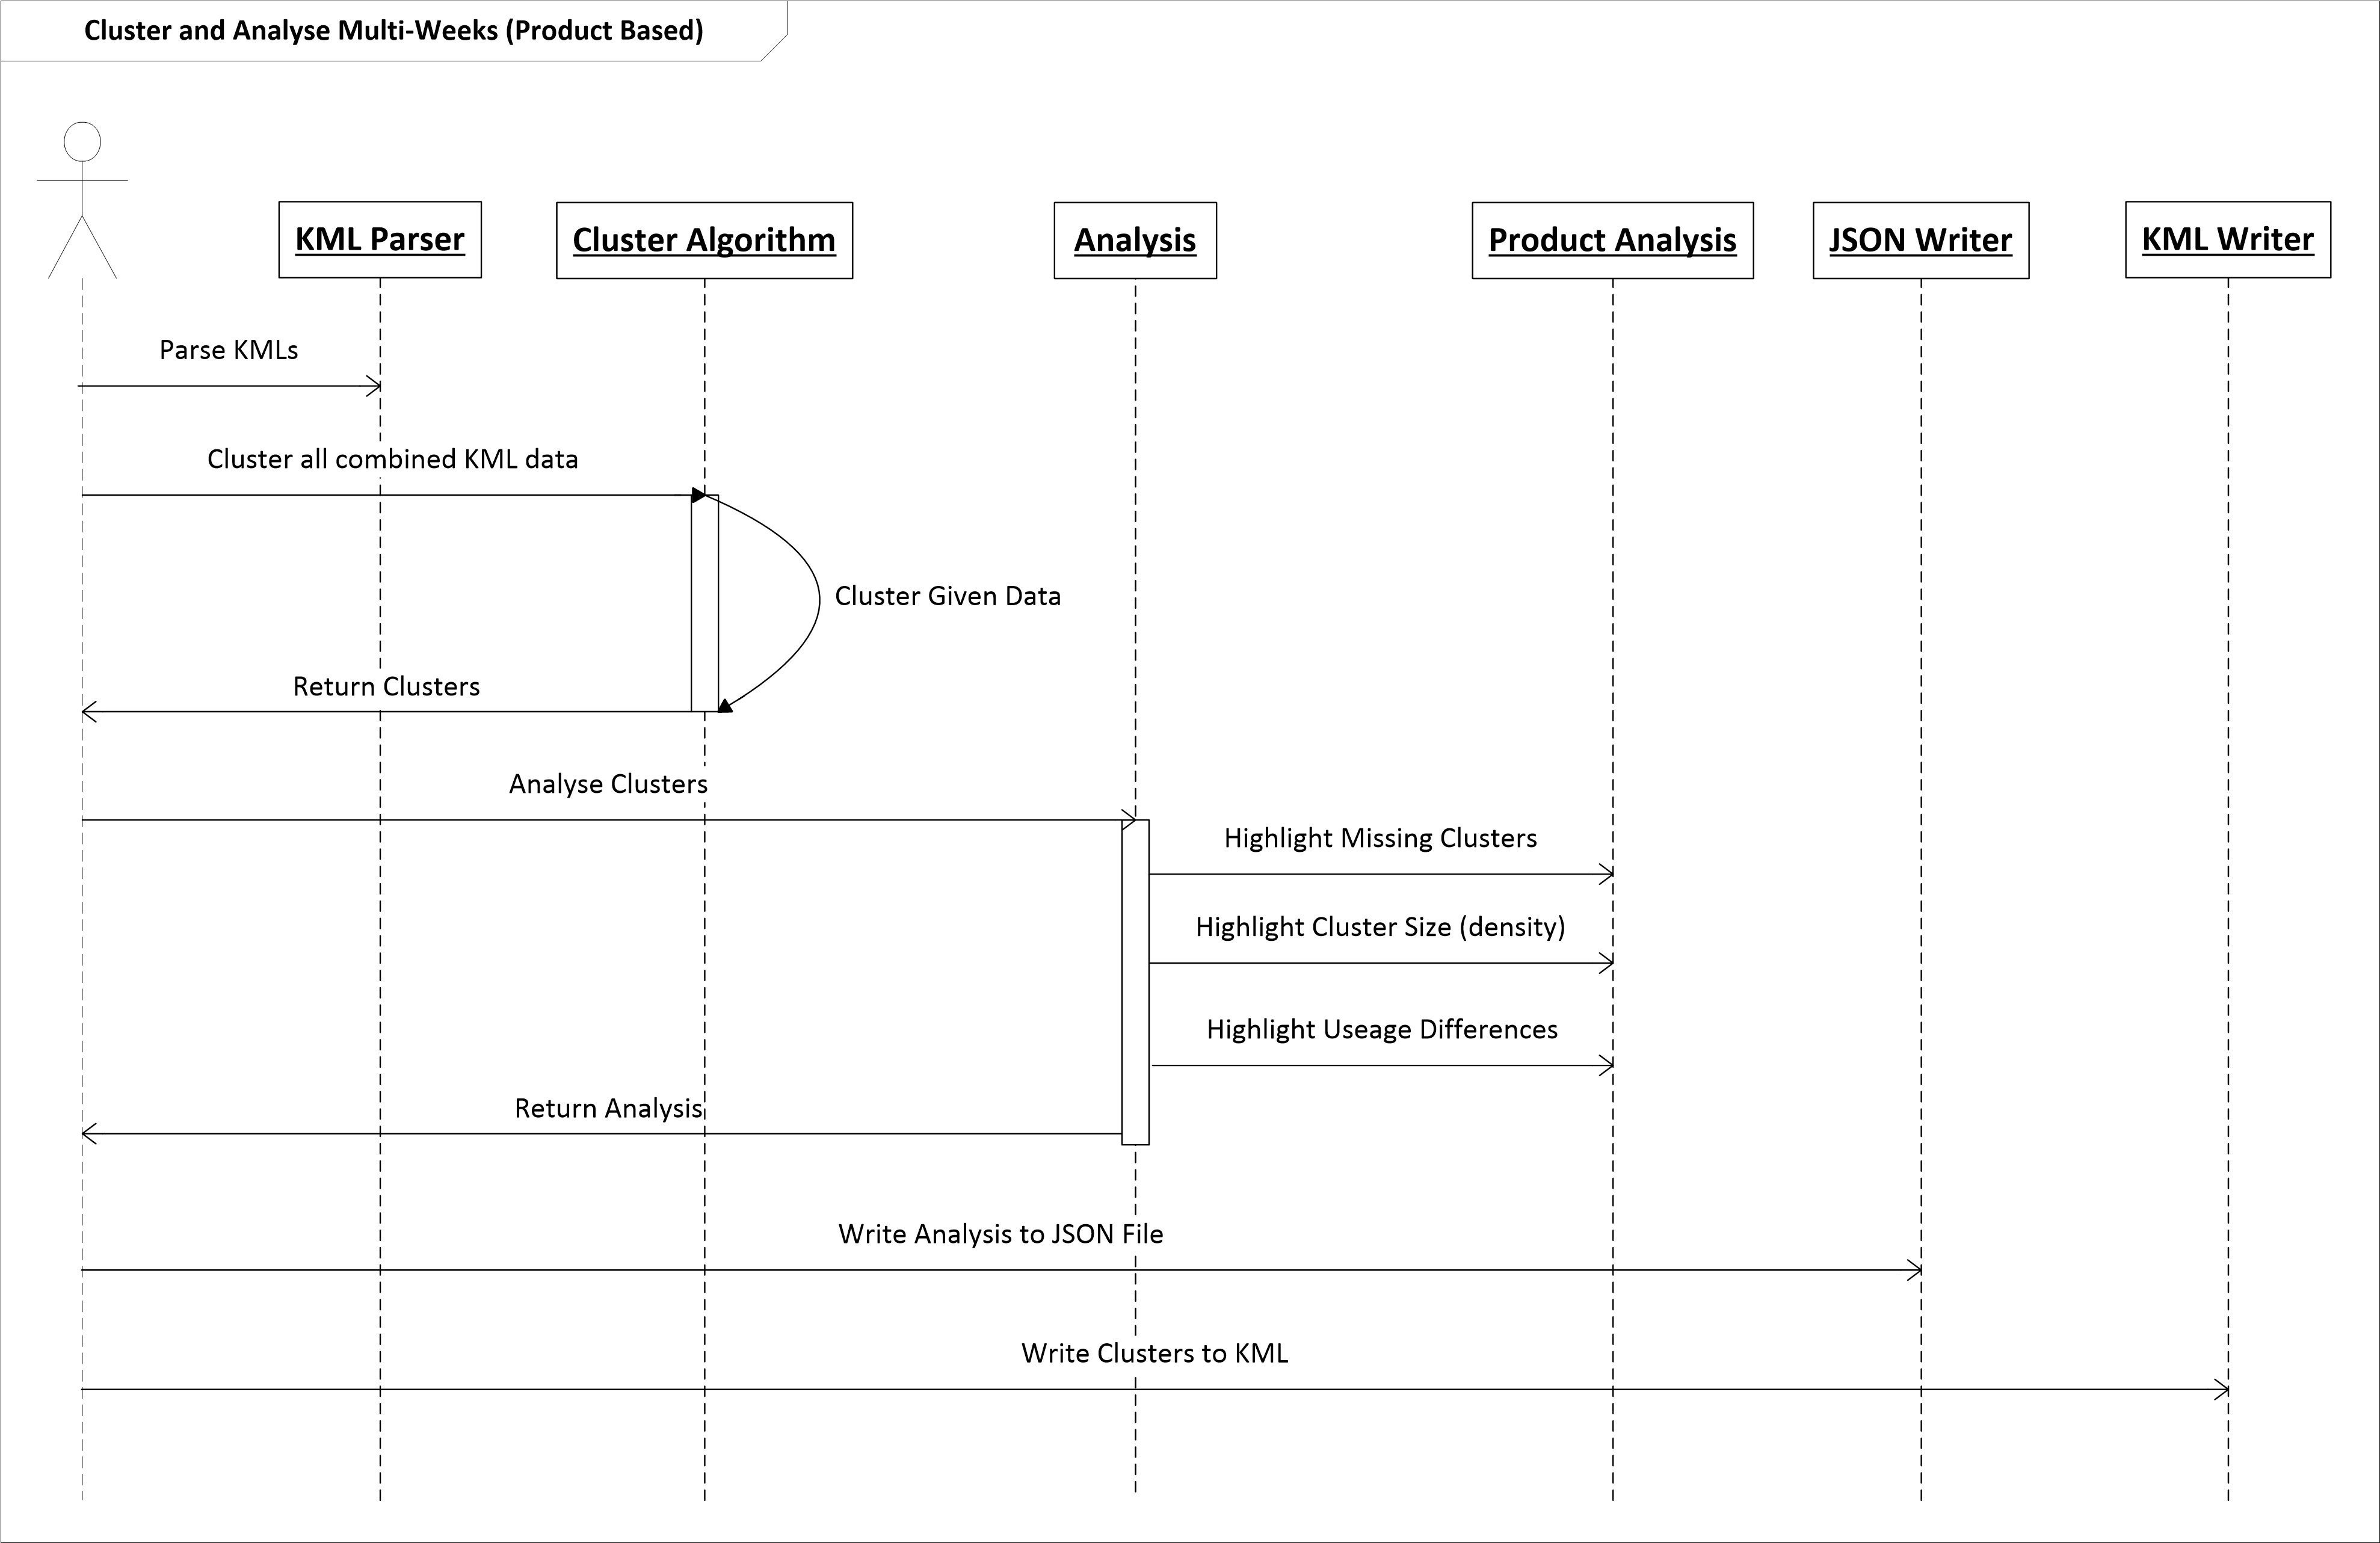
\includegraphics[scale=0.75]{chapter7/sequence_diagrams/multi_week_cluster_product.png}
        \caption[Sequence diagram of a multi-week being clustered]
                {Sequence diagram of a multi-week being clustered and analysed 
                upon a product basis.}
        \label{fig:multiproduct}
    \end{figure}
  \end{landscape}
  % Flush page
  \clearpage
}

